\documentclass{standalone}
\usepackage{tikz} % Import the tikz package
\usetikzlibrary{automata} % Import library for drawing automata
\usetikzlibrary{positioning} % ...positioning nodes
\usetikzlibrary{arrows} % ...customizing arrows
\tikzset{node distance=2.5cm,
    every state/.style={
        semithick,
        fill=gray!10},
    initial text={},
    double distance=2pt,
    every edge/.style={
        draw,
        ->,>=stealth',
        auto,
        semithick}}
\let\epsilon\varepsilon
\begin{document}
    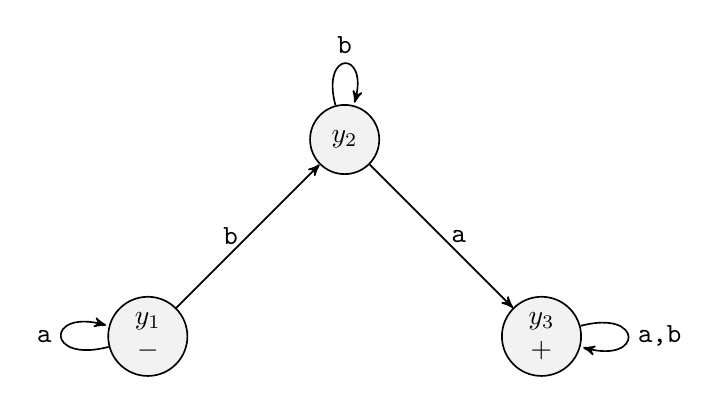
\begin{tikzpicture}
        \node[] (mid) {};
        \node[state,left of=mid,align=center] (y1) {$y_1$\\$-$};
        \node[state,above of=mid] (y2) {$y_2$};
        \node[state,right of=mid,align=center] (y3) {$y_3$\\$+$};

        \draw (y1) edge[loop left] node {\tt a} (y1);
        \draw (y1) edge[left] node {\tt b} (y2);

        \draw (y2) edge[loop above] node {\tt b} (y2);
        \draw (y2) edge[right] node {\tt a} (y3);

        \draw (y3) edge[loop right] node {\tt a,b} (y3);
    \end{tikzpicture}
\end{document}